% Shared standalone design for the editable figure reconstructions.
\documentclass[tikz,border=5pt,10pt]{standalone}
\usepackage[T1]{fontenc}
\usepackage[utf8]{inputenc}
\usepackage{newpxtext,newpxmath}
\usepackage[scaled=.94]{sourcesanspro}
\usepackage{pgfplots}
\pgfplotsset{compat=1.18}
\usetikzlibrary{arrows.meta,calc,positioning,decorations.pathreplacing,
  decorations.markings,patterns,matrix,shapes.geometric,fit,backgrounds,
  intersections,angles,quotes}
\definecolor{ink}{HTML}{203746}
\definecolor{accent}{HTML}{146C78}
\definecolor{muted}{HTML}{667780}
\definecolor{signalred}{HTML}{B94B44}
\color{ink}
\tikzset{>=Latex,line width=.8pt,
  every node/.style={font=\small},
  axis/.style={->,draw=muted,line width=.5pt},
  guide/.style={draw=muted,dashed,line width=.45pt},
  curve/.style={draw=accent,line width=1pt},
  marker/.style={circle,fill=accent,inner sep=1.5pt},
  labelbox/.style={fill=white,inner sep=2pt}}

\begin{document}
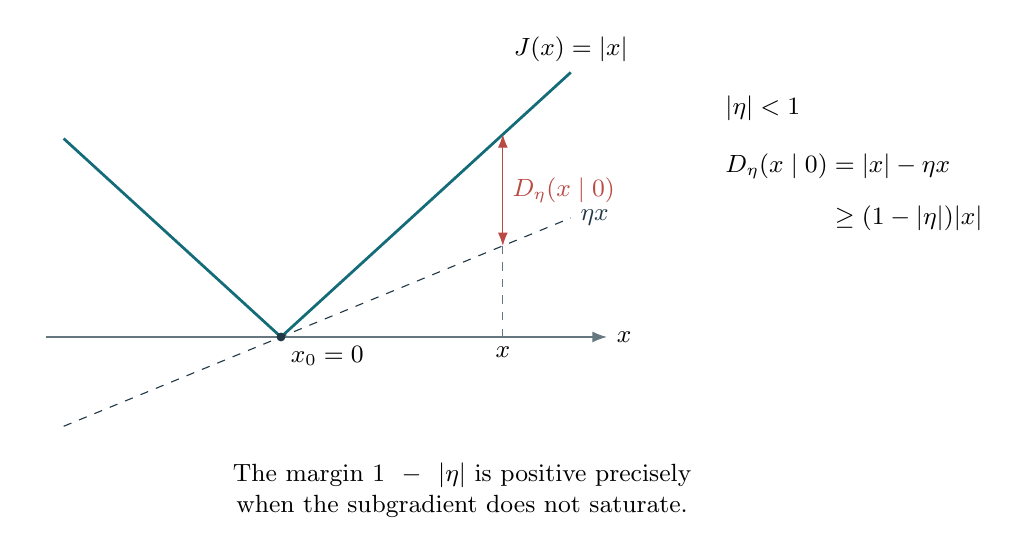
\begin{tikzpicture}[x=1.15cm,y=1.05cm]
\draw[axis](-2.6,0)--(3.6,0)node[right]{$x$};
\draw[curve](-2.4,2.4)--(0,0)--(3.2,3.2)node[above]{$J(x)=|x|$};
\draw[ink,dashed](-2.4,-1.08)--(3.2,1.44)node[right]{$\eta x$};
\node[below right]at(0,0){$x_0=0$};\fill[ink](0,0)circle(1.6pt);
\draw[guide](2.45,0)node[below]{$x$}--(2.45,1.1025);
\draw[<->,signalred](2.45,1.1025)--(2.45,2.45)node[midway,right]{$D_\eta(x\mid0)$};
\node[anchor=west,align=left]at(4.8,2.1){$|\eta|<1$\\[10pt]$D_\eta(x\mid0)=|x|-\eta x$\\[8pt]$\phantom{D_\eta(x\mid0)}\geq(1-|\eta|)|x|$};
\node[align=center,text width=10.8cm]at(2,-1.85){The margin $1-|\eta|$ is positive precisely when the subgradient does not saturate.};
\end{tikzpicture}
\end{document}
